\capitulo{4}{Técnicas y herramientas}

En esta sección se describirán tanto las herramientas como las metodologías utilizadas, necesarias para la elaboración del proyecto. En la tabla 4.1 aparecen listadas todas las tecnologías.



\tablaSmall{Herramientas y tecnologías utilizadas en cada parte del proyecto.}{l c c c c}{herramientasportipodeuso}{ \multicolumn{1}{l}{Herramientas} & WebApp ReactJS & API & BD & Memoria \\}{ 
REACTJS & X & & &\\
OPENLAYERS & X & & &\\
BOOTSTRAP & X & & &\\
JAVASCRIPT & X & & &\\
REACT-ROUTER-DOM & X & & &\\
ZUSTAND & X & & &\\
P5 & X & & &\\
SASS & X & & &\\
JANUS & X & & &\\
NGINX & X & & &\\
OPENAPI & & X & &\\
PYTHON & & X & &\\
FLASK & & X & &\\
SQLALCHEMY & & X & &\\
MYSQL & & & X &\\
LATEX & & & & X\\
OVERLEAF & & & & X\\
TeXMaker & & & & X\\
DOCKER & & X & X &\\
JSON & X & X & &\\
GIT+GITHUB & X & X & X & X\\
}{t}



\section{Metodologías}
\subsection{Scrum}
Con el uso de esta metodología ágil se consiguió hacer un desarrollo incremental e iterativo de la aplicación, mediante el uso de \textit{sprints} siendo estos los ejes de desarrollo del proyecto.

\section{Patrones de diseño}
\subsection{MODELO VISTA CONTROLADOR (MVC)}
Es un modelo de arquitectura de sistemas utilizado en la parte de la API para la gestión de los datos con la interfaz de usuario.
Se compone de tres partes principales:

\begin{itemize}
    \item \textbf{Modelo}: Es la parte del modelo que se encarga de la lógica de negocio y de la persistencia.
    \item \textbf{Vista}: Esta parte esta formada por los datos enviados al cliente y todas las formas de interacción con ellas.
    \item \textbf{Controlador}: Es la parte que hace de intermediario entre la parte de la Vista y el Modelo generando un flujo de datos y modificándolos para adaptarlo a cada una de las partes si es necesario.
\end{itemize}

En la figura 4.1 podemos ver un esquema que representa la interacción de las distintas partes del modelo \textit{MVC}.
\begin{figure}[t]
    \centering
    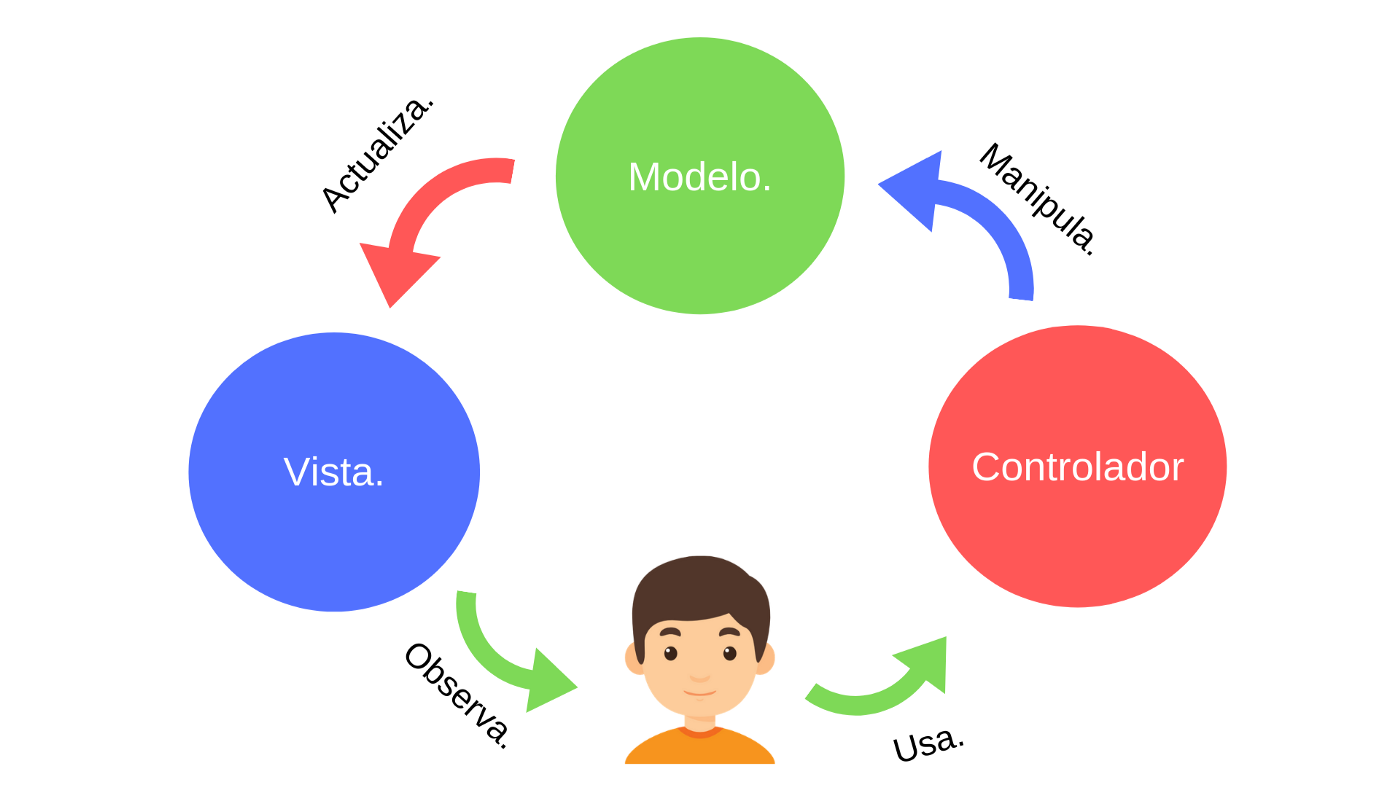
\includegraphics[width=10cm,height=10cm,keepaspectratio]{img/mvc.png}
    \caption{Imagen de \textit{MVC} \cite{mvcImag}.}
    \label{fig:imagen-mvc}
\end{figure}





\subsection{Arquitectura del sistema}

En nuestro caso teniendo en cuenta el modelo \textit{MVC}\cite{mvc}:

\begin{itemize}
\item La parte del \textbf{modelo} estaría en la \textit{API} y se encargaría de crear las bases de datos mediante el \textit{ORM SQLAlchemy}, así como también de generar todas las relaciones entre las tablas. También genera un esquema de cada tabla para poder hacer operaciones con los datos.\item La parte del \textbf{controlador} también estaría en la \textit{API}, teniendo la lógica de interacción, con otras partes del sistema, en cada llamada a los \textit{endpoints}.
\item En \textbf{vista} podríamos considerar la parte de la \textit{webapp} que interactúa mediante los \textit{endpoints} con la \textit{API} para luego mostrar los datos que recibe o hacer operaciones en la base de datos.
\end{itemize}

Podemos ver el esquema general del proyecto en la figura 4.2.

\FloatBarrier
\begin{figure}[h]
    \centering
    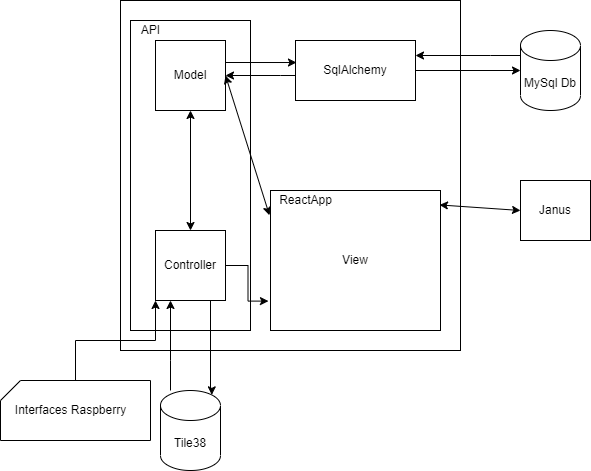
\includegraphics[width=10cm,height=10cm,keepaspectratio]{img/Esquema general del proyecto.drawio (1).png}
    \caption{Esquema del sistema.}
    \label{fig:Esquema-del-sistema}
\end{figure}
\FloatBarrier

\subsection{Maestro-Esclavo}
Esta arquitectura es utilizada principalmente en las \textit{raspberries} cuando queremos escalar el sistema para localizar a usuarios en habitaciones grandes. Tendríamos una \textit{raspberry} maestra que pediría la información a las \textit{raspberries} esclavas, y sería la maestra la que controlaría la información. Al no tener entornos grandes, en este proyecto, solo se han utilizado \textit{raspberries} con rol maestro.

Tendríamos un concepto similar llamado \textit{Follower-Leader}, utilizado en \textit{Tile38}, que es un sistema de \textit{geofencing}, donde tenemos un contenedor con el rol de \textit{Leader} y otro con el rol de \textit{Follower}, así el acceso a los recursos es mucho más rápido.
\section{Control de versiones}
\subsection{GIT}
Se ha utilizado \textit{git} como herramienta de control de versiones, haciendo un registro de versiones mediante \textit{commits} y \textit{branches}, y usando repositorios locales y remotos.
\subsection{GITHUB}
Github es una plataforma de desarrollo colaborativo en la nube, que hace uso de la herramienta \textit{git} alojando código en el repositorio remoto asignado.
\section{Entorno de desarrollo}
\subsection{Visual Studio Code}
\textit{Visual Studio Code} es un editor de código que viene con la herramienta \textit{git} integrada, viene con soporte nativo para lenguajes como \textit{Javascript} y acceso rápido a cualquiera de sus librerías mediante predicción inteligente de escritura, así como soporte para lenguajes de marcas como \textit{HTML} u hojas de estilo como \textit{CSS}.

Este editor cuenta con una selección de \textit{plugins} de la comunidad que le hacen compatible para escribir código con muchísimos lenguajes del mercado.
\subsection{DBeaver}
Se ha utilizado \textit{DBeaver} como cliente de \textit{SQL}, esta herramienta ha sido muy útil durante el desarrollo del proyecto permitiendo consultar, escribir modificar o borrar datos y/o estructuras de las tablas en cualquier momento con una interfaz gráfica.
\section{Documentación}
\subsection{TeXMaker}
Es un procesador de texto multiplataforma que permite crear documentos en \LaTeX y exportarlo a diferentes formatos.
\subsection{Overleaf}
Procesador de texto colaborativo, online, que permite la escritura de documentos en \LaTeX y su exportación en diferentes formatos.
\section{Herramientas para el desarrollo}
\subsection{Docker}
Herramienta que permite la automatización del despliegue de distintos tipos de aplicaciones, funciona con contenedores que se basan en imágenes y proporciona una capa de abstracción para la virtualización de servicios.
\subsection{NGINX}
Herramienta que permite el despliegue de un servicio web, creando un servidor web que atiende peticiones.
En este proyecto esta herramienta se ha utilizado como \textit{reverse proxy} para atender peticiones por \textit{HTTPS }y redirigirlas a un dirección y puerto de la \textit{API} por \textit{HTTP} y desplegándola con \textit{docker}.
\subsection{MYSQL}
Sistema de gestión de bases de datos creada por \textit{Oracle}, el cual crea un servidor para dar servicio y que los clientes se conecten para poder interactuar con las tablas o con alguna base de datos.
\subsection{Javascript}
Lenguaje de programación orientado a cliente y se interpreta de manera nativa en los buscadores modernos.
\subsection{SaSS}
Tipo de lenguaje de hoja de estilos que añade más posibilidades que las hojas de estilos convencionales a la hora de programar, haciendo que las hojas de estilo de \textit{SaSS} sean fácil la tarea de mantener con grandes secciones de código.


\section{Librerías}
\subsection{ReactJS}
\textit{ReactJS} es una biblioteca de \textit{Javascript} creada por \textit{Facebook}, con la finalidad de crear aplicaciones de una sola página dinámicas.

Se basa en el concepto de componentes y estado. Donde un componente es una pieza de código, con similitudes a una clase en \textit{Java}, donde se definen e implementan los métodos, además tiene un método \textit{render}, de obligatoria llamada, que devuelve código \textit{jsx} muy similar a \textit{HTML}.\cite{React}

Un componente puede ser llamado por otro en la función \textit{render} como etiqueta, todo lo que se le pase como atributos será accesible como propiedades dentro del componente.

El estado del componente son todas aquellas variables que van a ser definidas para el propósito del componente, son constantes y se modifican a través de funciones implícitas de \textit{React}.

Existen dos tipos de componentes:
\begin{itemize}
    \item \textit{\textbf{Statefull Component}}: es un componente con estado, su responsabilidad es cambiar o mantener el estado, y pasarlo como atributos si es necesario.
    \item \textit{\textbf{Stateless Component}}: es un componente sin estado, solo muestra información estática o información pasada como propiedades.
\end{itemize}

Todo esto se ha modernizado en las últimas versiones de \textit{React} con la implementación de \textit{hooks}, que son métodos implícitos que utilizan el concepto de componentes de manera interna, simplificando el desarrollo tan rígido de los componentes.

Para la gestión de las páginas en \textit{React}, se utiliza una librería llamada \textit{react-router-dom}, que en el componente raíz, permite gestionar la ruta de la página y el componente a procesar por el buscador. El uso de esta librería hace que cambiar de página sea una simple llamada a la \textit{api} de la librería.

Además en algunas partes de la aplicación se requirió utilizar un estado compartido entre componentes independientes. Para esto se utilizó \textit{Zustand}, que es una librería que permite este funcionamiento. Este comportamiento no es recomendable en \textit{React}, ya que puede haber fugas de memoria, así que minimizamos el estado compartido lo máximo posible.
\subsection{React-router-dom}
Librería \textit{javascript open source} para controlar la navegación entre páginas de manera sencilla. Se basa en definir en el componente raíz unas rutas a las cuales podemos acceder con llamadas a la \textit{api} de la librería para representar gráficamente, en el buscador un componente a modo de página.
\subsection{Zustand}
Librería \textit{javascript open source} para poder tener un estado global accesible desde componentes independientes en \textit{React}.
\subsection{P5}
Librería \textit{javascript open source} para poder representar gráficamente objetos. Permite la posibilidad de desarrollar un sistema de dibujado, sobre un área concreta. En este trabajo se emplea para dibujar sobre las imágenes de las obras de arte que el visitante del museo está visualizando en su dispositivo. \cite{P5} 

Se basa en crear un \textit{canvas} de fondo, solo para la representación gráfica de una imagen, y posteriormente crear otro \textit{canvas} transparente encima, donde habilitaremos la opción de dibujar, pudiendo así dibujar encima de la imagen.

Esto se activará cuando la realidad aumentada detecte una obra de arte, y todo lo dibujado se guardará en la base de datos para su persistencia.

\subsection{OpenLayers}
Es una librería que se utiliza para la implementación de mapas. Su característica principal es que utiliza capas como unidad básica para la representación. Para que el objeto mapa identifique las capas, se utilizan los vectores que puede agrupar una o más \textit{features} como una capa que se visualiza en el mapa.

Las \textit{features} son objetos con la información mínima para la representación en el mapa. A estos objetos se les puede aplicar un estilo permitiendo cambiar, por ejemplo, la imagen a mostrar en el mapa.

En este proyecto para la representación del mapa se utiliza una capa tipo \textit{Tile}, y una capa \textit{Vector} agrupando todo el \textit{GeoJson} de la importación del edificio en la ubicación que queremos, siendo estas dos las capas principales.


Las capas de los \textit{tags} y \textit{anchors} son capas \textit{Vector} con un \textit{source} de un objeto \textit{Feature}. Sin embargo las \textit{Rooms} son capas \textit{Vector }con una \textit{source} de tipo \textit{Polygon}. Esto porque los \textit{tags} y \textit{anchors} se basan solo en una coordenada y las \textit{rooms} en varias. Todas estas coordenadas utilizadas se incluyen en una variable en formato \textit{geoJSON}, que es una porción de código con sintaxis \textit{JSON} pero que se utiliza para la representación de un objeto en el mapa.
\subsection{Bootstrap}
Librería \textit{open source} para la creación de interfaces web mediante el uso de hojas de cascada.
\subsection{Janus}
Librería basada en \textit{WebRTC} para el \textit{stream} de diferentes tipos de datos. En este proyecto se ha utilizado un \textit{docker} como servidor con un \textit{docker} y un cliente web \textit{javascript}.
\subsection{Flask}
\textit{Framework} de \textit{Python} que permite la creación de aplicaciones web. Esta herramienta se ha utilizado para la creación de \textit{endpoints} de la \textit{API} a modo de servidor con \textit{docker}.
\subsection{SQLAlchemy}
Herramienta que permite utilizar los datos de la base de datos como objetos en \textit{Python} permitiendo el llamado \textit{ORM (Object Relational Map)}.

\section{Estándares}
\subsection{JSON}
Estándar para el intercambio de datos entre servicios.
\subsection{GEOJSON}
Es un estándar de de representación geográfica de elementos sencillos. Está basada en formato \textit{JSON}, por lo que se puede enviar y persistir en formato de \textit{string} de manera simple. \cite{GeoJson}
\subsection{OPENAPI}
Estándar para la definición de \textit{API's}.

